\title{Unsupervised learning}

\subsection{Unsupervised learning}

In unsupervised learning, the task is to infer hidden structure from
unlabeled data, comprised of training examples $\{x_n\}$.

We demonstrate how to do this in Edward with an example.
The script is available
\href{https://github.com/blei-lab/edward/blob/master/examples/mixture_gaussian_collapsed.py}
{here}.


\subsubsection{Data}

Use a simulated dataset of 2-dimensional datapoints
$\mathbf{x}_n\in\mathbb{R}^2$.
\begin{lstlisting}[language=Python]
def build_toy_dataset(N):
  pi = np.array([0.4, 0.6])
  mus = [[1, 1], [-1, -1]]
  stds = [[0.1, 0.1], [0.1, 0.1]]
  x = np.zeros((N, 2), dtype=np.float32)
  for n in range(N):
    k = np.argmax(np.random.multinomial(1, pi))
    x[n, :] = np.random.multivariate_normal(mus[k], np.diag(stds[k]))

  return x

N = 500  # number of data points
D = 2  # dimensionality of data

x_train = build_toy_dataset(N)
\end{lstlisting}

We visualize the generated data points.
\begin{lstlisting}[language=Python]
plt.scatter(x_train[:, 0], x_train[:, 1])
plt.axis([-3, 3, -3, 3])
plt.show()
\end{lstlisting}
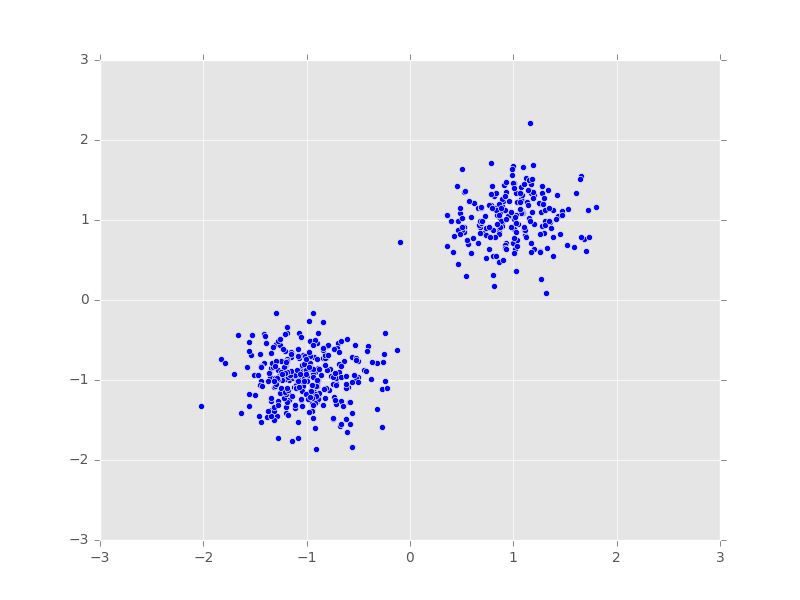
\includegraphics[width=700px]{/images/unsupervised-fig0.png}

\subsubsection{Model}

Posit the model as a mixture of Gaussians. For more details on the
model, see the
\href{/tutorials/mixture-gaussian}
{Mixture of Gaussians tutorial}.
We write it in collapsed form, marginalizing out
the mixture assignments.
\begin{lstlisting}[language=Python]
K = 2  # number of components

mu = Normal(mu=tf.zeros([K, D]), sigma=tf.ones([K, D]))
sigma = InverseGamma(alpha=tf.ones([K, D]), beta=tf.ones([K, D]))
cat = Categorical(logits=tf.zeros([N, K]))
components = [
    MultivariateNormalDiag(mu=tf.ones([N, 1]) * tf.gather(mu, k),
                           diag_stdev=tf.ones([N, 1]) * tf.gather(sigma, k))
    for k in range(K)]
x = Mixture(cat=cat, components=components)
\end{lstlisting}


\subsubsection{Inference}
Perform variational inference.
%
The latent variables are the mixture probabilities,
component means, and component variances.
Define the variational model to be
\begin{align*}
 q(\mu, \sigma \;;\; \lambda)
 &=
 \prod_{k=1}^K
 \text{Normal}(\mu_k; \lambda_{\mu_k})
 ~
 \text{InverseGamma}(\sigma_k; \lambda_{\sigma_k}).
\end{align*}
The model in Edward is
\begin{lstlisting}[language=Python]
qmu = Normal(
    mu=tf.Variable(tf.random_normal([K, D])),
    sigma=tf.nn.softplus(tf.Variable(tf.zeros([K, D]))))
qsigma = InverseGamma(
    alpha=tf.nn.softplus(tf.Variable(tf.random_normal([K, D]))),
    beta=tf.nn.softplus(tf.Variable(tf.random_normal([K, D]))))
\end{lstlisting}

Run variational inference for 4000 iterations and 20 latent variable
samples per iteration.
\begin{lstlisting}[language=Python]
inference = ed.KLqp({pi: qpi, mu: qmu, sigma: qsigma}, data={x: x_train})
inference.run(n_iter=4000, n_samples=20)
\end{lstlisting}
In this case
\texttt{KLqp} defaults to minimizing the
$\text{KL}(q\|p)$ divergence measure using the score function
gradient.
For more details on inference, see the \href{/tutorials/klqp}{$\text{KL}(q\|p)$ tutorial}.


\subsubsection{Criticism}

We visualize the predicted memberships of each data point.
We pick the cluster assignment which produces
the highest posterior predictive density for each data point.

To do this, we first draw a sample from the posterior and calculate a
a K x N matrix of log-likelihoods, one for each cluster assignment $k$
and data point $\mathbf{x}_n$. We perform this averaged over 100
posterior samples.
\begin{lstlisting}[language=Python]
# Average per-cluster and per-data point likelihood over many posterior samples.
log_liks = []
for _ in range(100):
  mu_sample = qmu.sample()
  sigma_sample = qsigma.sample()
  # Take per-cluster and per-data point likelihood.
  log_lik = []
  for k in range(K):
    x_post = Normal(mu=tf.ones([N, 1]) * tf.gather(mu_sample, k),
                    sigma=tf.ones([N, 1]) * tf.gather(sigma_sample, k))
    log_lik.append(tf.reduce_sum(x_post.log_prob(x_train), 1))

  log_lik = tf.pack(log_lik)  # has shape (K, N)
  log_liks.append(log_lik)

log_liks = tf.reduce_mean(log_liks, 0)
\end{lstlisting}

We then take the $\arg\max$ along the rows (cluster assignments).
\begin{lstlisting}[language=Python]
clusters = tf.argmax(log_liks, 0).eval()
\end{lstlisting}

Plot the data points, colored by their predicted membership.
\begin{lstlisting}[language=Python]
plt.scatter(x_train[:, 0], x_train[:, 1], c=clusters, cmap=cm.bwr)
plt.axis([-3, 3, -3, 3])
plt.title("Predicted cluster assignments")
plt.show()
\end{lstlisting}

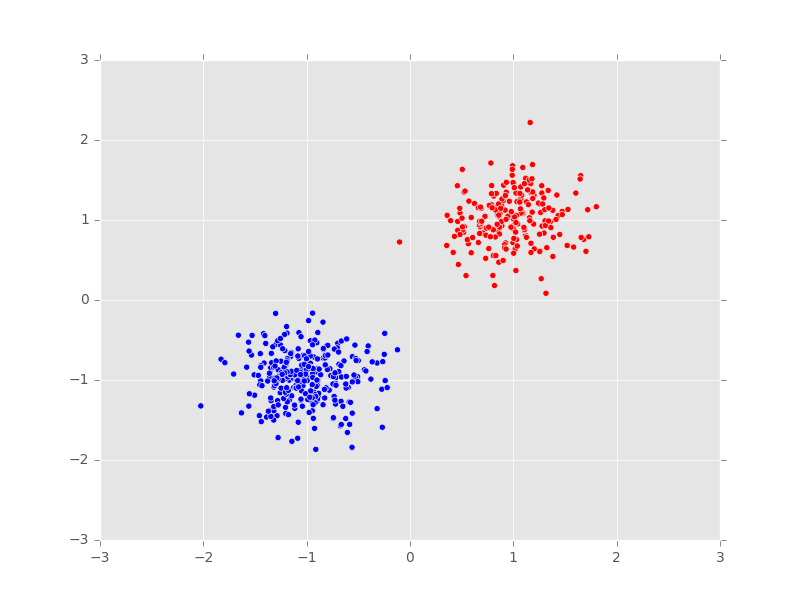
\includegraphics[width=700px]{/images/unsupervised-fig1.png}
